\documentclass[12pt]{article}
\usepackage{amsmath}
\usepackage{physics}
    \usepackage{graphicx}
\usepackage[linesnumbered,ruled,vlined]{algorithm2e}
\usepackage{listings} % Add this package to include code listings
\usepackage{xcolor} % Required for custom colors

% Define custom colors
\definecolor{codegreen}{rgb}{0,0.6,0}
\definecolor{codegray}{rgb}{0.5,0.5,0.5}
\definecolor{codepurple}{rgb}{0.58,0,0.82}
\definecolor{backcolour}{rgb}{0.95,0.95,0.92}

% Set up the style for Python code listings
\lstdefinestyle{pythoncode}{
    backgroundcolor=\color{backcolour},   
    commentstyle=\color{codegreen},
    keywordstyle=\color{magenta},
    numberstyle=\tiny\color{codegray},
    stringstyle=\color{codepurple},
    basicstyle=\ttfamily\footnotesize,
    breakatwhitespace=false,         
    breaklines=true,                 
    captionpos=b,                    
    keepspaces=true,                 
    numbers=left,                    
    numbersep=5pt,                  
    showspaces=false,                
    showstringspaces=false,
    showtabs=false,                  
    tabsize=2,
    language=Python % Specify the language for syntax highlighting
}

% Apply the style to Python listings
\lstset{style=pythoncode}
\author{Patryk Kozlowski}
\title{G0W0}
\date{\today}
\begin{document}
\maketitle
\section{The Fock Operator}
We are first interested in This can be easily later switched to the MO basis with something like $F_{pq} = \sum_{\mu} \sum_{\nu} C_{\mu p}^{*}F_{\mu\nu}C_{\nu q}$ where $C$ is the matrix of MO coefficients? an expression for the Fock operator in the AO basis. This can be easily later switched to the MO basis with something like $F_{pq} = \sum_{\mu} \sum_{\nu} C_{\mu p}^{*}F_{\mu\nu}C_{\nu q}$ where $C$ is the matrix of MO coefficients? Unfortunately, this seems to be giving diagonal element that are unreasonably large, so what could I be doing wrong? 
The Fock operator is defined in the AO basis using the density matrix. Does this mean that my Fock matrix in the AO basis is incorrect? 
\begin{equation}
F_{\mu\nu} = h_{\mu\nu} + \sum_{\lambda\sigma}P_{\lambda\sigma}(\mu\nu|\lambda\sigma) - \frac{1}{2}\sum_{\lambda\sigma}P_{\lambda\sigma}(\mu\lambda|\nu\sigma)
\end{equation}
where $h_{\mu\nu}$ is the one-electron Hamiltonian (in the AO basis, this is just mf.get\_hcore?), $P_{\lambda\sigma}$ is the density matrix, and $(\mu\nu|\lambda\sigma)$ is the two-electron repulsion integral all in AO basis.
\subsection{density matrix}
The density matrix is defined as
\begin{equation}
P_{\mu\nu} = 2\sum_{i=1}^{N/2}C_{\mu i}C_{\nu i}^{*}
\end{equation}
where $C$ is the matrix of MO coefficients. I want to convince myself that the above identity is indeed true and I can do this using mf.mo\_coeffs(:, :n\_occupied) for $C$ and mf.get\_rdm1() for $P$. Indeed this is true! I am finding that playing around with the elements of the Fock procedure is hopeful for my understanding of what is going on.
\subsection{Electron Repulsion Integrals in the AO Basis}
Is this the proper way to get them?
\begin{lstlisting}[language=Python]
eri_ao = molecule.intor('int2e').reshape((n_orbitals, n_orbitals, n_orbitals, n_orbitals))
\end{lstlisting}
\section{Getting rid of the python loops}
In 
\begin{equation}
    A_{iajb}=\delta _{ij} \delta _{ab} \left(\varepsilon _{a}-\varepsilon _{i}\right) + 2(ia|jb)
\end{equation}
the latter term is easy enough to get into np.einsum notation. The first term is a bit more difficult. I need to think about this some more. I have
\begin{lstlisting}[language=Python]
occupied_energies = orbital_energies[:n_occupied]
virtual_energies = orbital_energies[n_occupied:]
\end{lstlisting}
so I think I am on the right track, but I am not sure where to go from here.
And then I have something like this
\begin{equation}
    \Sigma_{pp}^{\text{correlation}}(\omega) = \sum_{\mu }^{\text{RPA}}\left(\sum_{j}^{\text{occupied}} \frac{V_{pj}^{\mu }V_{pj}^{\mu }}{\omega -(\varepsilon _{j}-\Omega  _{\mu })}+ \sum_{b}^{\text{virtual}} \frac{V_{pb}^{\mu }V_{bp}^{\mu }}{\omega -(\varepsilon _{b}+\Omega  _{\mu })}\right)
\end{equation}
can I get rid of for loops with this one, or am I out of luck?
\subsection{What to do about the $\varepsilon_{j}$ when I have a non-diagonal $F_{pq}^{HF}[\gamma^{DFT }]$}
and then I know that $F^{HF}[\gamma _{DFT}]$ is not diagonal, so what do I do whenever an orbital energy, like $\varepsilon _{j}$, appears, in equations 3 or 4, for example? I know that in my iterative procedure, for
\begin{equation}
    \delta_{pq}F_{pq}^{HF}[\gamma^{DFT }] + \Sigma_{p}^{corr}(\varepsilon_{p}^{QP}) = \varepsilon_{p}^{QP}
\end{equation}
I can use the diagonal of $F_{pq}^{HF}[\gamma^{DFT }]$ regardless of whether this matrix is diagonal. What do I do for the $\varepsilon_{j}$ though in 3 or 4? Do I diagonalize $F_{pq}^{HF}[\gamma^{DFT }]$ and then use the diagonal elements of that matrix?

\section{Changing To dRPA}
If I recall correctly, I have something like
\begin{equation}
    \begin{pmatrix}
    A & B \\
    -B & -A
    \end{pmatrix}
    \begin{pmatrix}
    X \\
    Y
    \end{pmatrix}
    =
    \begin{pmatrix}
    X \\
    Y
    \end{pmatrix}
    E
\end{equation}
where $A$ is 
\begin{equation}
    A_{iajb}=\delta _{ij} \delta _{ab} \left(\varepsilon _{a}-\varepsilon _{i}\right) + 2(ia|jb)
\end{equation}
and $B$ is
\begin{equation}
    B_{iajb} = 2(ia|bj)
\end{equation}
I am not sure about the form for $B$, so correct me if I am wrong.\\
This seems to be an eigenvalue problem with an ndim = 4 tensor, so how would i solve? Because equation 6 seems like an eigenvalue problem for a tensor with shape $(2, 2, \mu, \mu)$ which I am not familiar with solving yet.



\section{Notation in Literature}
\subsection{Feynman Diagrams}
I notice that these are also used heavily in the literature as well. Could you recommend a text that would enable me to learn more about this? I guess there are many other things that I could be working on, so is this worth learning at this point?
\subsection{Standard Terms}
\begin{figure}[h]
    \centering
    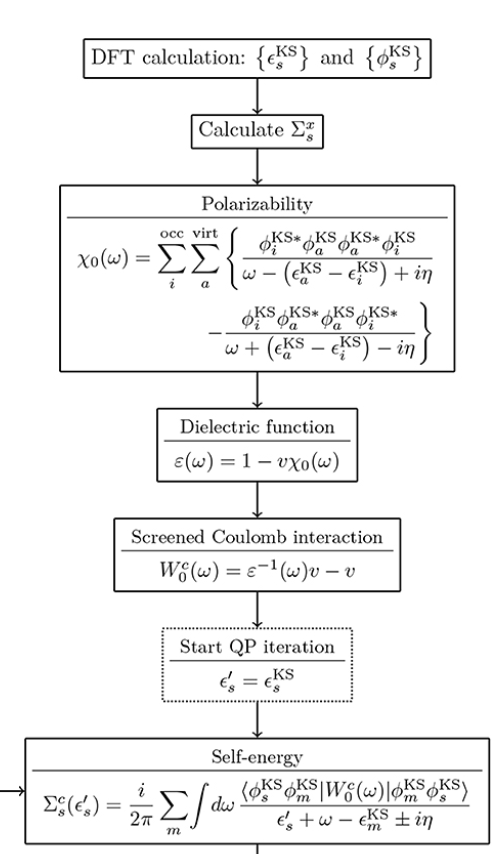
\includegraphics[width=0.8\textwidth]{not}
\end{figure}
And then I also see the $G_0$ term thrown around. I see elements of these in my current implementation, but will I understand more when I move to the RPA or is it more related to me dealing with the real part of the correlation self energy now (i.e. things would make more sense if this quantity was complex)? Some of these terms are in the image below.

\end{document}